% +---------------------------------------------------------------+
% | Author :    Noémie Plancherel, HEIG-VD
% | Date :      16.10.2022
% +---------------------------------------------------------------+

\chapter{KeePass}
\label{ch:keepass}

Ce chapitre sera dédié à l'analyse sécuritaire de l'application KeePass. Nous allons utiliser l'application desktop sur Windows 11. KeePass fonctionne entièrement en local et aucune donnée ne transitent sur le cloud. 

Nous voulons préciser que KeePass est open-source, ce qui va nous permettre d'analyser le code en cas de vulnérabilités trouvées. De  plus, cela nous permettra de proposer une correction du code afin de contribuer au gestionnaire de mots de passe.

\section{Environnement}

\begin{table}[H]
	\centering
	\begin{tabular}{ll}
		\hline
		Logiciel           & Version        \\ \hline
		Windows 11         & 10.0.22621     \\
		KeePass & 2.52       \\ \hline
	\end{tabular}
	\caption{Environnement utilisé pour KeePass}
\end{table}

Pour cette analyse, nous allons utiliser KeePass sans plugin supplémentaire, afin d'analyser l'application basique sans aucun ajout. Nous procédons de cette manière-ci car il existe beaucoup de plugins différents qui permettent d'ajouter des fonctionnalités différentes, comme des backups, une couche sécuritaire supplémentaire, de l'export, etc\footnote{\href{https://keepass.info/plugins.html}{https://keepass.info/plugins.html}}. Cependant, chaque plugin est développé par des personnes externes à KeePass, ainsi il est préférable de ne pas les inclure dans le rapport.

De plus, KeePass propose deux versions de son application, une 1.x et une 2.x. La première propose beaucoup moins de fonctionnalités et est moins flexible que la deuxième, c'est pour cela que nous nous basons sur la deuxième.
\section{Critères d'analyse}

L'établissement des critères d'analyse se basent sur l'analyse de menaces effectuée plus tôt dans le travail et sur les failles connues de KeePass afin qu'on puisse se baser dessus.

\begin{itemize}
	\item Master password
	\item Choix cryptographiques
	\begin{itemize}
		\item Chiffrement
		\item Dérivation des clés
		\item Authentification
	\end{itemize}
	\item Fonctionnalités proposées
	\begin{itemize}
		\item Génération de mots de passe
		\item Presse-papier
	\end{itemize}
	\item Stockage
	\item Mémoire
\end{itemize}

\section{Master password}

Quand l'utilisateur créée sa nouvelle base de données, où toutes les données du coffre-fort seront stockées dessus, KeePass demande de fournir un master password qui permettra d'y dériver la master de key et de chiffrer le coffre-fort. 

Il n'y a pas de critères exigés par KeePass lors de la spécification, ainsi l'utilisateur pourrait ajouter un seul caractère et le master password serait validé. Néanmoins, KeePass indique qu'il s'agit d'un mot de passe faible, ce qui pourrait permettre d'éviter des master password trop faibles qui permettrait d'effectuer une attaque de brute-force:

\begin{figure}[H]
	\centering
	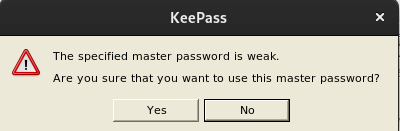
\includegraphics[width=8cm]{images/kp_weak.png}
	\caption{Avertissement de master password faible de KeePass}
\end{figure}

Le gestionnaire indique également la qualité du mot de passe en indiquant le nombre de bits d'entropie et la force du mot de passe. 

Il existe également des "options d'expert" qui permettent d'ajouter deux facteurs supplémentaires lors de la connexion. L'utilisateur peut fournir un \textit{key file} qui est un fichier qui contient une clé. Il est possible d'ajouter le compte utilisateur Windows (si on est sur cette OS), ce qui permet de faire la base de données dépendante à l'utilisateur connecté. De ce fait, il sera uniquement possible d'ouvrir le coffre-fort si on est connecté avec cet utilisateur. 

Pour chaque facteur ajouté, KeePass avertit \textbf{explicitement} que si on perd accès au facteur ou qu'on l'oublie, il est impossible de récupérer la base de données. Ainsi, ils conseillent de faire des backups pour le \textit{key file} et que leur emplacement soit différent que celui du coffre-fort.

Donc, il n'existe aucun critère minimal exigé lors de la création du coffre-fort. Cependant, dans une entreprise par exemple, les administrateurs ont la possibilité de modifier le fichier de configuration et d'ajouter une taille et la qualité du master password minimum. 

Un point très important à citer est qu'il est possible de ne pas configurer de master password, mais d'uniquement paramétrer soit un \textit{key file} soit le \textit{Windows Account User} soit les deux. Ainsi, cela pourrait être critique car un attaquant peu récupérer facilement le fichier avec la clé si ce dernier n'est pas dans un emplacement sécurisé et pour l'option de l'utilisateur Windows, si ce dernier est connecté sur la session de l'utilisateur, il pourra déverrouiller systématiquement le coffre-fort.

Bien que KeePass avertisse l'utilisateur qu'il a un master password trop faible, il serait recommandé d'ajouter une exigence quant à la qualité du mot de passe afin de s'assurer qu'il est fort. Car un particulier qui n'a pas ou peu de connaissances en sécurité informatique, il ne connaîtra pas les vulnérabilités liées à un mot de passe faible. Néanmoins, le fait que le gestionnaire est en uniquement en local, cela permet de freiner des attaques.

Il serait également recommandé de demander de toute manière un master password à l'utilisateur et de lui permettre d'ajouter des facteurs supplémentaires (comme le \textit{key file} par exemple).

\subsection{Brute-force authentification}

Lorsque l'utilisateur doit entrer le master password de son coffre-fort, étant donné que KeePass fonctionne en local, un attaquant aurait la possibilité d'effectuer du brute-force du master password en testant toutes les possibilités possibles. 

En testant plusieurs entrées incorrectes, nous avons remarqué que KeePass bloque le formulaire après 3 essais faux et ainsi afin de pouvoir retenter d'entrer le master password, il est nécessaire de ré-ouvrir la base de données ou de redémarrer l'application. 

Cette méthode ne stoppe pas les attaquants mais permet de les freiner considérablement car des manipulations sont nécessaires après seulement 3 essais. 
\section{Choix cryptographiques}
\subsection{Chiffrement}
La version 2.x de KeePass propose deux algorithmes de chiffrement; AES-CBC 256 et ChaCha20 256. Ces deux algorithmes sont recommandés et sont jugés comme très sécurisés\cite{ecrypt}. 

L'IV utilisé pour chiffrer le coffre-fort est généré aléatoirement et stocké dans le header du fichier de la base de données. L'aléatoire permet ainsi de chiffrer plusieurs coffre-forts avec la même master key. Pour l'initialiser, KeePass utilises un CPRNG (cryptographically secure pseudorandom number generator)\footnote{Algorithme déterministe qui vise à générer une séquence de nombre imprévisibles pour un adversaire}. Chaque générateur a besoin d'une source d'entropie pour l'initialiser, ainsi le gestionnaire crée une piscine d'entropie de différentes sources (notamment des nombres aléatoires générés par le fournisseur cryptographique du système, la date/heure actuelle et l'heure de mise en service, la position du curseur, etc.) afin d'avoir la meilleure entropie possible.

De plus, à chaque fois que la base de données est sauvegardée, c'est-à-dire si l'utilisateur a ajouté, modifié ou supprimé des entrées, un nouvel IV aléatoire est généré. 
\subsection{Dérivation des clés}
Pour la dérivation de la master key, nous nous référons au schéma réalisé et expliqué plus tôt dans le travail \ref{schema_keepass}. Nous remarquons que premièrement chaque facteur de connexion est hashé avec SHA-256 afin de créer une entrée (des données) pour la fonction de dérivation. La fonction de hachage SHA-256 est considéré comme sécurisée et recommandée dans le futur par ECRYPT. KeePass supporte deux algorithmes de dérivation de clés:

\textbf{AES-KDF} : par défaut, KeePass propose 60'000 itérations, qui sont modifiables par l'utilisateur. En sachant que plus il y d'itérations, plus les attaques par dictionnaires sont complexes, ce nombre est suffisant. 

\textbf{Argon2} : le gestionnaire propose deux variantes de cet algorithme: Argon2d et Argon2id. Le premier protège mieux contre les attaques GPU, alors que le deuxième protège mieux contre les \textit{side-channel attacks}\footnote{Attaque qui recherche et exploite des failles dans l'implémentation, logicielle ou matérielle du système}. Cette fonction est plus recommandée que AES-KDF car elle offre une meilleure résistance contre les attaques GPU et c'est un algorithme moderne (2015).

Puis la sortie des fonctions de dérivation est ensuite concaténée avec un sel aléatoire puis compressée avec SHA-256 afin de créer la clé finale, la master key.

Cette méthode permet d'amener une grande protection contre les attaques par dictionnaire et les attaques par guessing. Plus les paramètres des fonctions de dérivation ont des valeurs élevées, plus la clé sera difficile et prendra du temps à deviner pour un attaquant. 
\subsection{Authentification}
Comme expliqué dans la section \ref{local}, KeePass authentifie le header et les données du coffre-fort\cite{kdbx}. Le header authentifié à l'aide de HMAC-SHA-256 et est stocké directement après le header. Cela permet de vérifier que le fichier n'a pas été corrompu. De plus, un hash SHA-256 est stocké dans la base de données afin de vérifier que le header n'a pas été involontairement corrompu, sans connaître la master key.  

Les données du coffre-fort sont authentifiées à l'aide d'un hash HMAC-SHA-256. KeePass sépare toutes les données du coffre-fort en blocs de 1 MB, ainsi chaque bloc chiffré est authentifié. Le schéma utilisé est \textit{Encrypt-then-MAC}, qui est un schéma recommandé et qui permet de garantir l'intégrité des données claires et chiffrées. Le hash du bloc est généré avec les données chiffrées du bloc et une clé qui est différente pour chaque bloc, afin d'éviter toute réutilisation de clé. La clé pour HMAC est générée à l'aide de : $K_i := SHA-512(i ‖ K)$ où $K$ est une clé de 512 bits dérivée de la master key et du master seed (stocké dans le header du fichier KDBX).
\section{Fonctionnalités proposées}
\subsection{Génération de mots de passe}

Comme pour l'analyse de LastPass, nous allons également analyser la fonctionnalité de génération de mots de passe de KeePass\cite{pw}. Nous allons juger la force des mots de passe générés afin de garantir une bonne sécurité des entrées ajoutées par l'utilisateur. 

KeePass propose la génération suivante :

\begin{table}[H]
	\centering
	\resizebox{\textwidth}{!}{\begin{tabular}{llll}
		\hline
		Longueur supportée & Composition par défaut      & Taille par défaut & Symboles proposés              \\ \hline
		> 1              & {[}A-Za-z0-9{]} & 20                & !"\#\$\%\&'()*+,-./:;<=>?@[\textbackslash]\textasciicircum\_`\textbraceleft\textbraceright\texttildelow| \\ \hline
	\end{tabular}}
	\caption{Fonctionnalités de KeePass pour la génération de mots de passe}
\end{table}

Par défaut, KeePass ajoute au minimum un caractère par set de caractères choisi, ce qui permet de générer un mot de passe plus aléatoire. En plus de tous les sets de caractères proposés, il est possible d'inclure des caractères supplémentaires pour s'assurer qu'ils soient présents dans la génération de mots de passe par exemple. Presque tous les caractères Unicode sont supportés par Keepass\footnote{\href{https://keepass.info/help/base/pwgenerator.html\#charset}{https://keepass.info/help/base/pwgenerator.html\#charset}}. Cela permet d'avoir une grande variation de caractères différents, ce qui est un bon point pour la génération et l'aléatoire des mots de passe. 

D'autres modes de générations sont également disponibles (comme l'ajout de règles de génération), mais nous ne nous concentrerons pas dessus pour cette partie. 

Ainsi, nous allons effectuer les mêmes tests qu'avec LastPass en reprenant les mêmes compositions de mots de passe afin de pouvoir faire une comparaison entre les deux gestionnaires. Le pool de données suivant ont été généré:

\begin{itemize}
	\item lettres majuscules / minuscules (ll)
	\item lettres majuscules / minuscules + chiffres (lc)
	\item lettres majuscules / minuscules + symboles (ls)
	\item symboles + chiffres (sc)
	\item lettres majuscules / minuscules + symboles + symboles (all)
\end{itemize}

Nous avons également générer 10'000 mots de passe aléatoire par composition avec 12, 16 et 20 caractères pour évaluer leur robustesse. 

Afin de récupérer tous les mots de passe générés par KeePass, nous avons utilisé un plugin, proposé par KeePass. L'outil \textit{KPScript}\footnote{\href{https://keepass.info/help/v2\_dev/scr\_index.html}{https://keepass.info/help/v2\_dev/scr\_index.html}} permet d'effectuer du scripting avec KeePass. Il existe la fonctionnalité de \textit{single command} où il est possible d'utiliser le plugin comme commande et où la fonctionnalité de génération de mots de passe est disponible. Le point avantageux est qu'il existe un paramètre \textit{count} qui permet de générer \textit{n} mots de passe. Le second paramètre \textit{profile} permet de définir des profils de génération de mots de passe, par exemple, 12 caractères avec des majuscules et minsucles. 

Voici la commande utilisée pour générer 10'000 mots de passe avec une composition all : 
\begin{lstlisting}[language=bash,caption=Génération de mots de passe sur KeePass]
$ KPScript -c:GenPw -count:100000 -profile:"all"
\end{lstlisting}

Pour tester l'aléatoire et la robustesse des mots de passe, nous prenons le même script que pour LastPass \ref{script_test_last}, qui pour rappel utilise un outil \textit{zxcvbn} qui permet d'évaluer la force du mots de passe et du nombre d'essais qu'un attaquant aura besoin pour le deviner. Ce dernier évalue le nombre d'essais en fonction de 4 attaques différentes (voir section \ref{lp_pw}). L'échelle d'évaluation de la génération est également la même (pour des questions de redondance, se référer au chapitre LastPass).

Pour les résultats \ref{kp_result}, nous constatons qu'en moyenne, les mots de passe générés sont bons. KeePass génère rarement des mots de passe un peu plus faibles que d'autres, néanmoins même ceux qui sont considérés plus faibles, ont un bon score contre les différentes attaques. 

Étant donné que KeePass propose beaucoup de symboles différents dans sa génération, les mots de passes générés qui en possèdent sont forts. Et ainsi, contrairement à LastPass, les mots de passes faibles ne dépendent pas vraiment de leur composition de caractères, nous remarquons que les résultats varient. 

Au niveau du nombre de caractères, pour 12 caractères nous remarquons que les mots de passes sont fortement protégés contre les attaques en ligne, néanmoins un peu moins contre les attaques hors-ligne qui indiquent que pour des fonctions de hachage rapide, il faudrait moins de 3 secondes pour deviner le mot de passe. Dès 16 caractères, nous remarquons une meilleure protection au niveau des attaques hors-ligne, cependant ils sont modérément protégés contre les attaques avec hachage rapide. Pour 20 caractères, n'importe quel mot de passe, même un peu plus faible, et suffisamment protégé contre toute attaque.

Vu que KeePass est open-source, nous avons inspecté le code afin d'observer comment l'aléatoire dans les mots de passe était géré. Nous voyons qu'un stream de nombre aléatoire est créé :

\begin{lstlisting}[style=c, caption=Fonction \textit{CreateRandomStream} de KeePass]
private static CryptoRandomStream CreateRandomStream(byte[] pbAdditionalEntropy, out byte[] pbKey)
{
	pbKey = CryptoRandom.Instance.GetRandomBytes(128);
	// Mix in additional entropy
	Debug.Assert(pbKey.Length >= 64);
	if((pbAdditionalEntropy != null) && (pbAdditionalEntropy.Length > 0))
	{
		using(SHA512Managed h = new SHA512Managed())
		{
			byte[] pbHash = h.ComputeHash(pbAdditionalEntropy);
			MemUtil.XorArray(pbHash, 0, pbKey, 0, pbHash.Length);
		}
	}
	return new CryptoRandomStream(CrsAlgorithm.ChaCha20, pbKey);
}
\end{lstlisting}

\begin{lstlisting}[style=c, caption=Constructeur \textit{CryptoRandomStream} de KeePass]
public CryptoRandomStream(CrsAlgorithm a, byte[] pbKey)
{
	if(pbKey == null) { Debug.Assert(false); throw new ArgumentNullExceptuon("pbKey"); }
	inr cbKey = pbKey.Length;
	if(cbKey <= 0) 
	{
		Debug.Assert(false); // Need at least one byte
		throw new ArgumentOutOfRangeException("pbKey");
	}
	m_crsAlgorithm = a;
	if(a == CrsAlgorithm.ChaCha20)
	{
		byte[] pbKey32 = new byte[32]:
		byte[] pbIV12 = new byte[12];
		using(SHA512Managed h = new SHA512Managed())
		{
			byte[] pbHash = h.ComputeHash(pbKey);
			Array.Copy(pbHash, pbKey32, 32);
			Array.Copy(pbHash, 32, pbIV12, 0, 12);
			MemUtil.ZeroByteArray(pbHash);
		}
	m_chacha20 = new ChaCha20Cipher(pbKey32, pbIV12, true);
	}
	[...]
}
\end{lstlisting}

L'algorithme ChaCha20 est utilisé comme un CSPRNG (\textit{cryptographically secure pseudorandom number generator}), car il est possible d'utiliser des algorithmes \textit{stream cipher} pour ce genre de générateur\cite{random}. En suivant les recommandations du NIST\cite{SP80090A} concernant les générateurs de nombres aléatoires, les étapes suivantes sont recommandées:

\begin{itemize}
	\item \textbf{Entropie} consiste à récupérer de l'entropie afin de pouvoir créer la seed aléatoire. KeePass va récupérer l'entropie de l'utilisateur de plusieurs sources différentes. 
	\item \textbf{Seed} est utilisée pour instantier le CSPRNG et par la suite générer des bits aléatoires. Afin de la créer, il est recommandé d'utiliser une fonction de hachage afin de compresser les bits d'entropie récupérés précédemment. Dans le premier extrait de code, SHA-512 est utilisé pour compresser les bits. Il est également recommandé d'utiliser un nonce en plus de l'entropie, nous voyons que KeePass génère 128 bits aléatoires en supplément. 
	\item \textbf{Re-seeding} cette partie est importante car elle permet de rafraîchir le pool d'entropie interne. Générer trop de sorties d'une même seed pourrait fournir suffisamment d'informations afin de prédire avec succès les futures sorties. Dans le second extrait du code, KeePass prend comme paramètre la seed précédente et la hache à nouveau avec SHA512. Cependant, elle ne prend pas en paramètre l'entropie de l'utilisateur, ce qui est recommandé par le NIST.  
	\item \textbf{Génération} la dernière étape consiste à créer le générateur afin de récupérer des valeurs aléatoires. Le générateur est créé à l'aide de l'initialisation d'un cipher. Pour ce gestionnaire, ChaCha20 est utilisé pour générer les bits aléatoires. La clé est changée à chaque fois qu'un mot de passe est généré afin de garantir qu'une future clé compromise ne mette pas en danger des sorties précédentes. De plus, nous remarquons que le tableau qui contient la seed et qui n'est plus utilisé est effacé de la mémoire afin de s'assurer qu'aucun attaquant puisse y avoir accès et deviner les prochaines sorties du générateur.
\end{itemize}

Dernièrement, sur KeePass, chaque caractère du mot de passe est généré en appelant le cipher ChaCha20 créé précédemment. 

Il est mieux d'utiliser des \textit{stream ciphers} au lieu d'utiliser des fonctions PRNG/DRBG (l'algorithme Blum Blum Shub par exemple qui est uniquement utilisé pour la génération de nombres aléatoires), car ils permettent d'être plus simples à implémenter et plus rapides. 

\subsection{Presse-papier}

Pour évaluer la sécurité de la fonctionnalité de presse-papier sur KeePass, nous allons effectuer plusieurs analyses différentes. Premièrement, nous allons expliquer comment le gestionnaire gère cette fonctionnalité, puis nous allons effectuer quelques tests et finalement, nous allons analyser le code de l'application. 

Dans la version la plus récente, par défaut, KeePass nettoie le presse-papier après 12 secondes et nettoie également le contenu copié dès que KeePass est fermé. Ces deux options permettent d'amener une grande sécurité quant au sniffing de presse-papier par exemple. Le nombre de secondes est paramétrable, cependant 12 secondes est un nombre très suffisant. 

De plus, une autre option activée par défaut demande à KeePass de ne pas stocker les éléments copiés dans l'historique de Windows. Une sécurité supplémentaire est également implémentée à propos des applications tierces de presse-papier, l'option \textit{Use Clipboard Viewer Ignore clipboard format} permet à des applications d'ignorer le contenu copié par KeePass, car certaines sauvegardent le contenu du presse-papier et empêche de pouvoir le nettoyer. 

Ainsi, nous avons effectué les tests suivants :
\begin{itemize}
	\item[\checkmark] Copier un mot de passe et tester si le contenu du presse-papier était nettoyé
	\item[\checkmark] Copier un mot de passe et contrôler qu'il soit bien effacé de l'historique de Windows 11
	\item[\checkmark] Copier un mot de passe, verrouiller le gestionnaire et contrôler que le mot de passe soit effacé du presse-papier après 12 secondes
	\item[\checkmark] Copier un mot de passe, fermer l'application et vérifier que rien ne soit stocké dans le presse-papier
	\item[\checkmark] Copier un mot de passe, copier un autre élément externe à KeePass avant les 12 secondes et vérifier que le mot de passe ne soit pas stocké dans l'historique de Windows
	\item[\checkmark] Copier un mot de passe, verrouiller le gestionnaire, copier un autre élément externe à KeePass avant les 12 secondes et vérifier que le mot de passe ne soit pas stocké dans l'historique de Windows
\end{itemize}

Tous les tests ci-dessous ont été testés et ont tous été passés avec succès. Cela signifie que la fonctionnalité du presse-papier est très bien gérée par KeePass et qu'elle garantie une grande sécurité vis-à-vis de cette dernière. Néanmoins, le risque n'est pas à zéro, car un attaquant aurait toujours la possibilité d'ajouter un malware sur le device de l'utilisateur qui permettrait de récupérer les éléments du presse-papier, mais il est difficile de se protéger complètement de ces attaques. 

Au niveau du code, en se référant au fichier \textit{ClipboardUtil.Windows.cs}, KeePass n'utilise que des méthode natives, c'est-à-dire qu'elle importe des fonctions de l'API Utilisateur Windows.

\begin{lstlisting}[style=c, caption=Importation des méthodes natives de l'API de Windows]
[DllImport("User32.dll", SetLastError = true)]
internal static extern IntPtr SetClipboardData(uint uFormat, IntPtr hMem);
\end{lstlisting}
Ci-dessous, un exemple d'importation que nous pouvons retrouver afin d'importer la copie de données dans le presse-papier. Ainsi, pour Windows, KeePass se base dans un premier temps sur les méthodes qui sont déjà proposées par l'OS, car elles fonctionnent efficacement. Toutefois, des fonctions implémentées par le développeur de KeePass sont proposées afin d'ajouter un support si les méthodes de Windows ne fonctionnent pas. 

\section{Stockage}

Étant donné que KeePass ne fonctionne qu'en local, le coffre-fort est stocké dans local sur l'appareil de l'utilisateur. Nous avons déjà expliqué comment KeePass gérait le coffre-fort \ref{kp_file}, néanmoins nous pouvons faire un bref rappel sur sa gestion. 

Tout le coffre-fort est stocké dans une base de données \textit{.kdbx} qui contient toutes les informations nécessaires quant à l'ouverture et le déchiffrement du coffre-fort. La base de données est séparée en deux parties; un header et un contenu. Le header contient tous les bytes pour la dérivation de la master key et le chiffrement des données. Le contenu quant à lui, contient des hashs pour l'authentification du header, afin d'éviter qu'il soit involontairement corrompu et qu'il ne soit pas authentique. Il contient également des blocs de données qui sont chacun authentifiés à l'aide d'un hash HMAC-SHA256 et qui sont chiffrés. Dès que tous les blocs sont déchiffrés à l'aide de la master key, les blocs sont concaténés et cela forme une base de données XML qui contient tout le coffre-fort en clair. 

La master key n'est jamais stockée dans la base de données pour éviter qu'un attaquant puisse la récupérer et déchiffrer toute la base de données, néanmoins si le master password est brute-forcé, l'attaquant peut récupérer le coffre-fort en clair. 

Ainsi, nous avons suivi les différentes attaques du blog de harmj0y \cite{crack} afin d'attaquer la base de données et récupérer le master password. Nous allons tester les attaques suivantes:

\begin{itemize}
	\item[--] \textbf{Attaque \#1} brute-force de master password
	\item[--] \textbf{Attaque \#2} déverrouiller le coffre-fort avec un facteur \textit{Windows User Account} activé
\end{itemize}

\textbf{Attaque \#1}

Dans cette partie, nous allons tenter de récupérer le master password du coffre-fort depuis la base de données. Hashcat 3.0.0\footnote{\href{https://hashcat.net/forum/thread-5559.html}{https://hashcat.net/forum/thread-5559.html}} propose un support pour les versions 1.x et 2.x de Keepass afin de craquer les hashs de ces derniers. Ainsi, afin d'extraire un hash de la base de données de KeePass compatible avec Hashcat, un outil John The Ripper, \href{https://fossies.org/linux/john/src/keepass2john.c}{keepass2john} a été développé. De ce fait, ce dernier prend en paramètres le fichier \textit{.kdbx} de la base de données. 

Premièrement, nous allons chercher une base de données à attaquer et le binaire de l'application sur le device de l'utilisateur, car elle peut être stockée dans n'importe quel emplacement. Soit on utilise une commande Powershell:

\begin{lstlisting}[language=PowerShell, caption=Commande Powershell pour chercher le fichier kdbx]
Get-ChildItem -Path C:\Users\ -Include @("*kee*.exe", "*.kdb*") -Recurse -ErrorAction SilentlyContinue | Select-Object -Expand FullName | fl
\end{lstlisting}

Soit, on cherche le fichier de configuration XML de KeePass où les chemins des différentes base de données sont indiqués (et tous les autres facteurs de connexion). Sur Windows, le fichier se trouve à \verb|C:\Users\user\AppData\Roaming\KeePass\KeePass.config.xml|.

Étant donné que l'outil John The Ripper a quelques années (2013) et n'a pas été mis à jour, il ne supporte que le chiffrement AES, et non ChaCha20 ou Argon2, nous avons donc configuré une base de données avec un master password faible et nous avons laissé les paramètres par défaut lors de la création de coffre-fort, qui sont AES. Nous avons décidé de configurer ces paramètres en se mettant au mieux dans la peau d'un particulier qui aurait peu de connaissances sur la cryptographie.

Dès que nous avons l'emplacement de la base de données, nous lançons l'outil de hash:

\begin{lstlisting}[style=bash, caption=Outil keepass2john]
$ keepass2john Database.kdbx
Database:$keepass$*2*60000*0*fba5a877bc4231428a6ac61bb0db5af6ac92b4ecdd2f35bcc4bd3de7f76ffdd9*30de72f912159a9a666e3a624546a09761e4a8932a531d2f56d36d3e08c07dc0*74e5d2fb309d9f3ef81d4fbf78562b91*31af5d12f9d189defa02193b8d4c2db3d3c7f6cdd95ae7d37552c7121848605c*5f36c21ec05f1d97be40c4ce64d2870f2f74392e0ca3acd40304afaa6c7461df
\end{lstlisting}

Et puis, on utilise Hashcat pour récupérer le master password. On utilise avec un dictionnaire afin de trouver plus rapidement le master password:

\begin{lstlisting}[style=bash, caption=Commande Hashcat]
$ hashcat -a 0 -m 13400 -o cracked_output.txt --outfile-format 2 CrackThis.hash rockyou.txt
Session..........: hashcat
Status...........: Cracked
Hash.Name........: KeePass 1 (AES/Twofish) and KeePass 2 (AES)
Hash.Target......: $keepass$*2*60000*222*6b4d1292a0c332f17dc1dfa744e24...37704b
Time.Started.....: Mon Dec  5 13:42:32 2022 (5 mins, 40 secs)
Time.Estimated...: Mon Dec  5 13:48:12 2022 (0 secs)
Guess.Base.......: File (rockyou.txt)
Guess.Queue......: 1/1 (100.00%)
Speed.#1.........: 284 H/s (14.02ms) @ Accel:256 Loops:128 Thr:1 Vec:8
Recovered........: 1/1 (100.00%) Digests
Progress.........: 96256/14344384 (0.67%)
Rejected.........: 0/96256 (0.00%)
Restore.Point....: 94208/14344384 (0.66%)
Restore.Sub.#1...: Salt:0 Amplifier:0-1 Iteration:59904-60000
Candidates.#1....: 431987 -> master10
\end{lstlisting}

Nous constatons que Hashcat a correctement cracké le master password et l'a trouvé en 5 minutes, ce qui est plutôt rapide. Néanmoins, le master password était \textit{password98}, ce qui est faible mais peut refléter le genre de mots de passe que les particuliers pourrait configurer. 

Finalement, l'attaquant connaît l'emplacement de la base de données et le master password, ainsi il peut la déverrouiller avec facilité. 

\textbf{Attaque \#2}

Cette attaque demande d'avoir quelques informations au préalable et est donc plus difficile à reproduire. Cette attaque permet à un attaquant, qui aurait pu récupérer la base de données de l'utilisateur, son master password à l'aide d'un keylogger et le mot de passe Windows de ce dernier. Si l'option de connexion \textit{Windows User Account} est activée, la personne malveillante ne pourra malheureusement pas ouvrir le coffre-fort. 

Nous allons premièrement expliquer comment KeePass utilise ce facteur de connexion afin de créer la master key de l'utilisateur. Il se sert du DPAPI (\textit{Windows Data Protection Application Programming Interface})\cite{dpapi}. C'est une interface qui propose des fonctions cryptographiques qui permettent de chiffrer / déchiffrer des données sensibles DPAPI appelées \textit{binary large objects} ou \textit{blob}\footnote{Données binaires stockées comme une seule entité}. Les clés DPAPI, dérivées du mot de passe et utilisées pour chiffrer la master key, sont stockées sous \verb|C:\Users\{username}\AppData\Roaming\Microsoft\Protect\{SID}|. La master key permet de chiffrer des données \textit{blob}.

Dans le code de KeePass, dans le fichier \textit{KcpUserAccount}, nous pouvons constater que KeePass créée une données protégées DPAPI à l'aide d'entropie, de l'utilisateur actuel et de données aléatoires. Ces données sont ensuite stockées dans un fichier \textit{ProtectedUserKey.bin} qui est localisé sous \verb|C:\Users\{username}\AppData\Roaming\KeePass\| sur Windows. 

Étant donné que des utilisateur de KeePass ont déjà perdu leur master key incluant leur compte Windows, une procédure complète a été expliquée afin de recover le facteur de connexion \textit{Windows User Account}\footnote{\href{https://sourceforge.net/p/keepass/wiki/Recover\%20Windows\%20User\%20Account\%20Credentials/}{https://sourceforge.net/p/keepass/wiki/Recover\%20Windows\%20User\%20Account\%20Credentials/}}, et ainsi déverrouiller leur coffre-fort. Nous n'allons pas décrire toute la procédure car elle est complexe, cependant un script implémenté par harmj0y automatise tout le processus\cite{restore_dpapi}. 

De ce fait, le script a besoin du répertoire avec le SID de l'utilisateur, le nom et le domain de l'utilisateur puis le fichier de KeePass \textit{ProtectedUserKey.bin}.

{-----} ajouter image script !!!

\section{Mémoire}

À propos de la gestion de la mémoire sur Keepass\cite{kp_memory}, comme nous l'avons également cité dans la section précédente, DPAPI est utilisé sur Windows afin de chiffrer les données sensibles en mémoire. KeePass considère que les données sensibles du coffre-fort sont la master key et les mots de passe des entrées. Ainsi, les usernames, les notes ou les URLs sont en clairs dans la mémoire du processus, car ces informations n'exposent pas des données importantes et sensibles. 

En se basant sur une étude de 2019 sur le management de secrets dans les gestionnaires de mots de passe\cite{iseexploit}, des mots de passe en clair sont exposés dans la mémoire du processus

outil keethief

\section{Récapitulatif de l'analyse}
-lors de l'inscription KeePass indique quelques indices/aides sur les attaques de mots de passe ou sur la sécurité en général. good point pour les particuliers. 